%% thesis.tex 2014/04/11
%
% Based on sample files of unknown authorship.
%
% The Current Maintainer of this work is Paul Vojta.
%
% https://math.berkeley.edu/~vojta/tex/ucbthesis-phd.html

\documentclass{ucbthesis}
\usepackage[dvipdfmx]{graphicx} % needs to be up top
\usepackage{bmpsize}
\usepackage{amsmath}
\usepackage{amssymb}
\usepackage[sorting=none]{biblatex}
\usepackage{color}
\usepackage{etoolbox}
\usepackage[hidelinks]{hyperref}
\usepackage[super]{nth}
\usepackage{notoccite}
\newcommand{\bo}{\mathbf\Omega}
\newcommand{\vecr}{\textbf{r}}
\newcommand{\sigt}{\Sigma_t}
\newcommand{\sigs}{\Sigma_s}

\newenvironment{psmallmatrix}
  {\left(\begin{smallmatrix}}
  {\end{smallmatrix}\right)}

\makeatletter
\let\oldcite\cite
\pretocmd{\listoffigures}{\def\cite{\ignorespaces\@gobble}}{}{}
\apptocmd{\listoffigures}{\let\cite\oldcite}{}{}
\makeatother

% To compile this file, run "latex thesis", then "biber thesis"
% (or "bibtex thesis", if the output from latex asks for that instead),
% and then "latex thesis" (without the quotes in each case).

% Double spacing, if you want it.  Do not use for the final copy.
% \def\dsp{\def\baselinestretch{2.0}\large\normalsize}
% \dsp

% If the Grad. Division insists that the first paragraph of a section
% be indented (like the others), then include this line:
% \usepackage{indentfirst}

\newtheorem{theorem}{Jibberish}

\bibliography{references}

\hyphenation{mar-gin-al-ia}
\hyphenation{bra-va-do}
\hyphenation{ACRONYM}

\begin{document}

% Declarations for Front Matter

\title{Advanced Nuclear Engineering for a Better World}
\author{Nancy Neutron}
\degreesemester{Spring}
\degreeyear{2049}
\degree{Doctor of Philosophy}
\chair{Professor Sofia Syntax}
\othermembers{
	Associate Professor Sally Slurm \\
	Professor Esther Electron
	}
\numberofmembers{3}
\field{Engineering -- Nuclear Engineering}
% Designated Emphasis -- this is optional, and rare
%\emphasis{Computational and Data Science and Engineering}
\campus{Berkeley}

\maketitle
% Delete (or comment out) the \approvalpage line for the final version.
\approvalpage
\copyrightpage

% (This file is included by thesis.tex; you do not latex it by itself.)

\begin{abstract}

% The text of the abstract goes here.  If you need to use a \section
% command you will need to use \section*, \subsection*, etc. so that
% you don't get any numbering.  You probably won't be using any of
% these commands in the abstract anyway.

\texttt{a\ b\ s\ t\ r\ a\ c\ t}

\end{abstract}


\begin{frontmatter}

% You can delete the \clearpage lines if you don't want these to start on
% separate pages.

\setcounter{secnumdepth}{3}
\setcounter{tocdepth}{3}

% to show paragraphs in ToC (good for an outline, stylistically ugly):
% \setcounter{secnumdepth}{4}
% \setcounter{tocdepth}{4}

\tableofcontents
\clearpage
\listoffigures
\clearpage
\listoftables

\begin{acknowledgements}

THANKS EVERYONE

\vspace{\fill}

\footnotesize{This material is based upon work supported under a prestigious
graduate fellowship as well as supported by the Department 
of Excellence under Award Number(s) 31337.}

\end{acknowledgements}

\end{frontmatter}

\pagestyle{headings}

% (Optional) \part{First Part}

\chapter{Introduction}

This chapter is the introduction.

\section{Motivation}

In this section, we motivate the work presented in the following chapter.

\section{Goals and Impacts}

Make the world a little bit better.

\section{The Neutron Transport Equation}

Here it is: \cite{dude}:

\begin{multline}
\bo \cdot \nabla \psi(\vecr,E,\bo) + \Sigma_t(\vecr,E) \psi(\vecr,E,\bo) =  \\
\int_0^\infty\int_{4\pi} \Sigma_s(\vecr,E'\rightarrow E,\bo'\cdot\bo)
\psi(\vecr,E',\bo')d\bo'dE' + Q(\vecr,E,\bo).
\label{time_ind_NTE}
\end{multline}

\noindent Equation \ref{time_ind_NTE} is difficult to solve.

\chapter{Background}

This chapter provides information relevant to the core parts of this research.

\section{Approaches to Nuclear Engineering}

\subsection{Experimental Methods}

\subsubsection{Beam Experiments}

\subsubsection{Reactor Measurements}

\paragraph{Gold Foil Experiments}\mbox{} \\

\paragraph{Thermal Measurements}\mbox{} \\

\subsection{Computational Methods}

\subsubsection{Parallel Computing}

Big computers are useful but difficult to use.

\paragraph{Shared Memory}\mbox{} \\

OpenMP is a good idea for the shared memory model.

\paragraph{Distributed Memory}\mbox{} \\

MPI might be better for working with distributed memory.

\section{Previous Work}

Many people have worked on nuclear engineering. Here we'll highlight important and relevant
work from the history of nuclear engineering.

\subsection{Important Experiments}

Many interesting experiments have been performed.

\subsubsection{CP-1}

Chicago Pile-1 (CP-1) was the world's first nuclear reactor.

\subsection{Important Software}

Software development has taken place as well.

\subsubsection{MCNP}

A lot of people use MCNP \cite{mcnp}. It is good practice to cite software.


\subsection{Other Notable Work}




\chapter{Method Description and Implementation}

This chapter will describe our methodology and how we went about it.

\section{Method}

We came up with some procedures.

\section{Implementation}

\textcolor{red}{We're still working through those procedures, so this section is in red
to remind us to update it later.}

\section{Caveats}

Always wear appropriate PPE!




\chapter{Test Cases and Results}

\section{Graphical Results}

Figure \ref{figs} depicts a fig.

\begin{figure}[!htb]
\centering
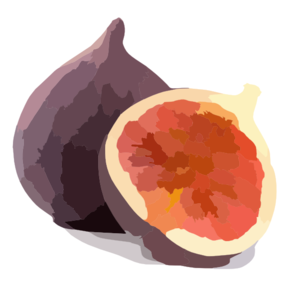
\includegraphics[width=0.5\textwidth]{img/whole-and-cut-fig-md.png}
\caption{A fig.}
\label{figs}
\end{figure}

\section{Tabulated Results}

In this section we tabulate results. Table \ref{tables} lists various types of
tables and Table \ref{numbers} lists some numbers.

\begin{table}[!htb]
\centering
\caption{Different types of tables.}
\begin{tabular}{cc}
\multicolumn{1}{c}{\textbf{Tables}} & 
\multicolumn{1}{c}{\textbf{Tables (cont'd)}} \\
\hline
Dining room & Coffee \\
Nightstand & Workbench 
\end{tabular}
\label{tables}
\end{table}

\begin{table}[!htb]
\centering
\caption{Some numbers.}
\begin{tabular}{|c|c|}
\hline
\multicolumn{1}{|l|}{\textbf{Positive}} & 
\multicolumn{1}{l|}{\textbf{Negative}} \\
\hline
5 & -40 \\
\hline
12 & -3 \\
\hline
\end{tabular}
\label{numbers}
\end{table}

\chapter{Conclusions and Future Work}

\begin{itemize}
\item{Results are pretty good!}
\item{We are kind enough to leave work for future students.}
\end{itemize}


\def\StripPrefix#1>{}
\def\jobis#1{FF\fi
  \def\predicate{#1}%
  \edef\predicate{\expandafter\StripPrefix\meaning\predicate}%
  \edef\job{\jobname}%
  \ifx\job\predicate
}

\if\jobis{thesis}
  \printbibliography
\else
  \newpage
  \renewcommand{\thepage}{}
  \printbibliography
\fi

%\appendix
% \include{mathbg}

\end{document}
